\documentclass[a4paper, 12 pt]{article}

\usepackage[english, russian]{babel}
\usepackage[T2A]{fontenc}
\usepackage[utf8]{inputenc}
\usepackage{graphicx}
\usepackage[unicode, pdftex]{hyperref}
\DeclareGraphicsExtensions{.png, .pdf}
\begin{document}
	\pagestyle{plain}
	\begin{center}
		\large МИНИСТЕРСТВО НАУКИ И ВЫСШЕГО ОБРАЗОВАНИЯ РОССИЙСКОЙ ФЕДЕРАЦИИ\
		\vspace*{5mm}
		
		\small ФЕДЕРАЛЬНОЕ ГОСУДАРСТВЕННОЕ АВТОНОМНОЕ ОБРОЗОВАТЕЛЬНОЕ УЧРЕЖДЕНИЕ ВЫСШЕГО ОБРАЗОВАНИЯ
		\mbox{\guillemotleft Национальный исследовательский институт ИТМО\guillemotright}
		\vspace*{10mm}
		
		\mbox{ФАКУЛЬТЕТ ПРОГРАМНОЙ ИНЖЕНЕРИИ И ВЫЧИСЛИТЕЛЬНОЙ ТЕХНИКИ}
		\vspace*{5mm}
		
		{\bf ЛАБОРАТОРНАЯ РАБОТА №2}
		\linebreak
		по дисциплине
		\linebreak
		\guillemotleft ИНФОРМАТИКА\guillemotright
		\linebreak
		\large Вариант №83
		\vspace*{50mm}
		
	\end{center}


	\begin{flushright}
		\textbf{\textit{Выполнил:}}
		\linebreak
		Студент группы P3118
		\linebreak
		Михайлов Дмитрий
		\linebreak
		Андреевич
		\linebreak
		\textbf{\textit{Преподаватель:}}
		\linebreak
		Рыбаков Степан
		\linebreak
		Дмитриевич
		\vspace*{30mm}
		
	\end{flushright}
	\begin{center}
		\small Санкт-Петербург, 2022
	\end{center}
	\thispagestyle{empty}
	\newpage
	\begin{flushleft}
		\textbf{\LARGE \section{Содержание}}
		\subsection{Задание........................................................3}
		\subsection{Основные этапы вычислений......................4 - 7}
		\subsection{Вывод...........................................................8}
		\subsection{Список литературы.....................................9}
	\end{flushleft}

	\newpage
	\begin{flushleft}
		\textbf{\LARGE 1.1 Задание.}
		\linebreak
		\LARGE Вариант №83
		\linebreak
		
		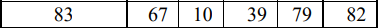
\includegraphics{screen1}
		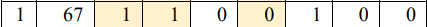
\includegraphics{screen2}
		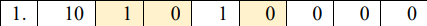
\includegraphics{screen3}
		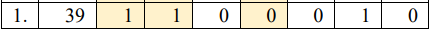
\includegraphics{screen4}
		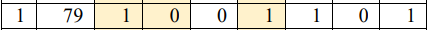
\includegraphics{screen5}
		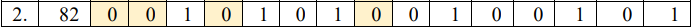
\includegraphics{screen6}
		
	\end{flushleft}

	\newpage
	\begin{flushleft}
		\textbf{\LARGE 1.2 Основные этапы вычислений.}
		\linebreak
		\textbf{а) Схема декодирования для (7; 4)}
		\linebreak
		\vspace*{10mm}
		
		\small Сначала переведём данные нам числа в 2-ую систему счисления.
		\linebreak
		\small а) $67_{10}$ = $1000011_{2}$
		\linebreak
		\small б) $10_{10}$ = $0001010_{2}$
		\linebreak
		\small в) $39_{10}$ = $0100111_{2}$
		\linebreak
		\small г) $79_{10}$ = $1001111_{2}$
		\vspace*{10mm}
		
		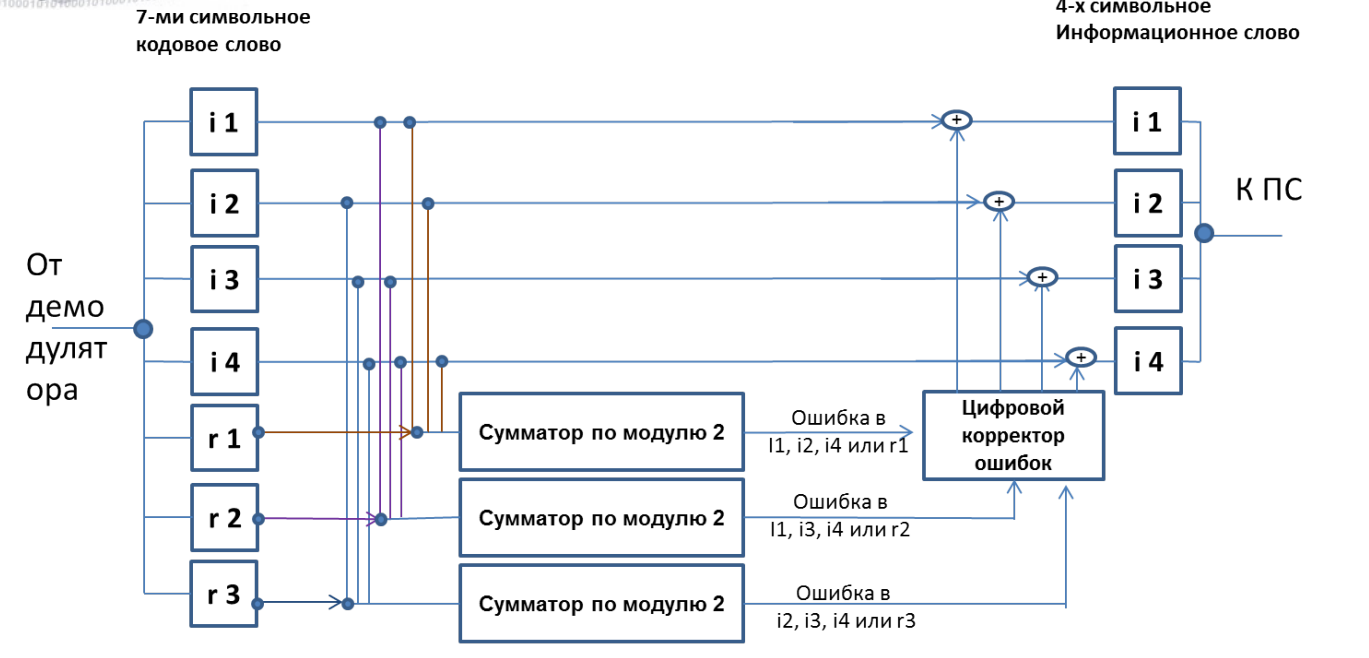
\includegraphics[width=10cm]{screen7}
		\linebreak
	\end{flushleft}

	\begin{flushleft}
		\small Для лучшего понимания схемы декодирования для классического кода Хэмминга(7; 4) построим таблицу, где каждый бит числа будет соответствовать своему значению:
	\end{flushleft}

	\begin{tabular}{|p{5mm}|p{5mm}|p{5mm}|p{5mm}|p{5mm}|p{5mm}|p{5mm}|p{5mm}|p{5mm}|}
		\hline
		& 1 & 2 & 3 & 4 & 5 & 6 & 7 & \\
		\hline
		$2^x$ & $r_1$ & $r_2$ & $i_1$ & $r_3$ & $i_2$ & $i_3$ & $i_4$ & S \\
		\hline
		1 & X & & X & & X & & X & $s_1$ \\
		\hline
		2 & & X & X & & & X & X & $s_2$ \\
		\hline
		4 & & & & X & X & X & X & $s_3$ \\
		\hline
	\end{tabular}
	\vspace*{5mm}
	
	\begin{flushleft}
		\small Значение синдромов будут вычисляться с помощью операции \textbf{сложения по модулю}:
		\linebreak
		$s_1$ = $r_1$ $\bigoplus$ $i_1$ $\bigoplus$ $i_2$ $\bigoplus$ $i_4$
		\linebreak
		$s_2$ = $r_2$ $\bigoplus$ $i_1$ $\bigoplus$ $i_3$ $\bigoplus$ $i_4$
		\linebreak
		$s_3$ = $r_3$ $\bigoplus$ $i_2$ $\bigoplus$ $i_3$ $\bigoplus$ $i_4$
		\linebreak
		
	\end{flushleft}

	\newpage
	\begin{flushleft}
		\small Тогда алгоритм вычисления позиции, где находиться ошибка, будет следующим:
		\linebreak
		\small 1) Развернуть конфигурацию.
		\linebreak
		\small 2) Перевести из 2-ой системы счисления в 10-ую.
		\linebreak
		\vspace*{5mm}
		
		\small a) Для числа 67 конфигурация синдромов($s_1$, $s_2$, $s_3$) будет 000, а это означает, что ошибки в этом сообщении не может быть.
		\linebreak
		\vspace*{5mm}
		
		\small б) Для числа 10 конфигурация синдромов($s_1$, $s_2$, $s_3$) будет 010, а это означает, что ошибка в бите 2, т.е. в $r_2$. Правильная запись будет такая - $0101010_2$
		\linebreak
		\vspace*{5mm}
		
		\small в) Для числа 39 конфигурация синдромов($s_1$, $s_2$, $s_3$) будет 011, а это означает, что ошибка в бите 6, т.е. в $i_3$. Правильная запись будет такая - $0100101_2$
		\linebreak
		\vspace*{5mm}
		
		\small г) Для числа 79 конфигурация синдромов($s_1$, $s_2$, $s_3$) будет 011, а это означает, что ошибка в бите 1, т.е. в $r_1$. Правильная запись будет такая - $0001111_2$
		\linebreak
	\end{flushleft}

	\newpage
	\begin{flushleft}
		\textbf{б) Схема декодирования для (15;11)}
		\linebreak
		\vspace*{10mm}
		
		\small Сначала переведём данное нам сообщение в 2-ую систему счислени, но длина должна быть равна 15 битам, то остальную часть забьём незначащими нулями.
		\linebreak
		\small д) $82_{10}$ = $000000001010010_2$
		\linebreak
		\vspace*{5mm}
		
		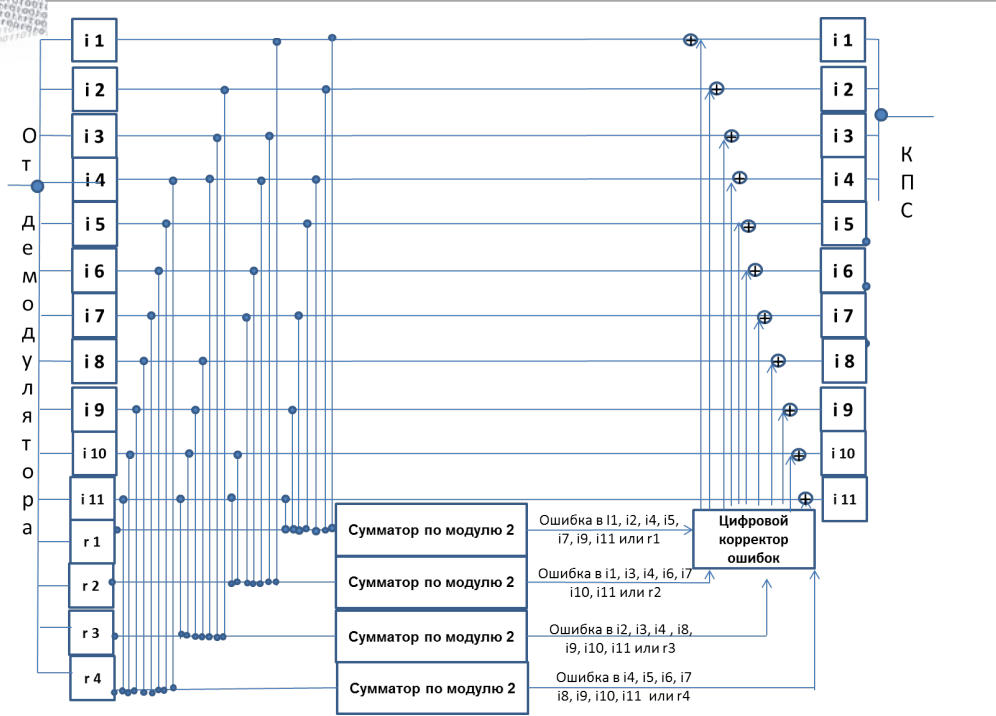
\includegraphics[width=10cm]{screen8}
		\vspace*{5mm}
		
		\small Для лучшего понимания схемы декодирования для классического кода Хэмминга(15; 11) построим таблицу, где каждый бит числа будет соответствовать своему значению:
		\linebreak
	\end{flushleft}

	\begin{table}[ht]
		\centering
		\begin{tabular}{|p{5mm}|p{5mm}|p{5mm}|p{5mm}|p{5mm}|p{5mm}|p{5mm}|p{5mm}|p{5mm}|p{5mm}|p{5mm}|p{5mm}|p{5mm}|p{5mm}|p{5mm}|p{5mm}|p{5mm}|}
			\hline
			& 1 & 2 & 3 & 4 & 5 & 6 & 7 & 8 & 9 & 10 & 11 & 12 & 13 & 14 & 15 & \\
			\hline
			$2^x$ & $r_1$ & $r_2$ & $i_1$ & $r_3$ & $i_2$ & $i_3$ & $i_4$ & $r_4$ & $i_5$ & $i_6$ & $i_7$ & $i_8$ & $i_9$ & $i_{10}$ & $i_{11}$ & S\\
			\hline
			1 & X & & X & & X & & X & & X & & X & & X & & X & $s_1$\\
			\hline
			2 & & X & X & & & X & X & &  & X & X & & & X & X & $s_2$\\
			\hline
			4 & & & & X & X & X & X & & & & & X & X & X & X & $s_3$\\
			\hline
			8 & & & & & & & & X & X & X & X & X & X & X & X & $s_4$\\
			\hline
		\end{tabular}
	\end{table}
	
	\newpage
	\begin{flushleft}
		\small Значение синдромов будут вычисляться с помощью операции \textbf{сложения по модулю}:
		\linebreak
		$s_1$ = $r_1$ $\bigoplus$ $i_1$ $\bigoplus$ $i_2$ $\bigoplus$ $i_4$ $\bigoplus$ $i_5$ $\bigoplus$ $i_7$ $\bigoplus$ $i_9$ $\bigoplus$ $i_{11}$		
		\linebreak
		$s_2$ = $r_2$ $\bigoplus$ $i_1$ $\bigoplus$ $i_3$ $\bigoplus$ $i_4$ $\bigoplus$ $i_6$ $\bigoplus$ $i_7$ $\bigoplus$ $i_{10}$ $\bigoplus$ $i_{11}$
		\linebreak
		$s_3$ = $r_3$ $\bigoplus$ $i_2$ $\bigoplus$ $i_3$ $\bigoplus$ $i_4$ $\bigoplus$ $i_8$ $\bigoplus$ $i_9$ $\bigoplus$ $i_{10}$ $\bigoplus$ $i_{11}$
		\linebreak
		$s_4$ = $r_4$ $\bigoplus$ $i_5$ $\bigoplus$ $i_6$ $\bigoplus$ $i_7$ $\bigoplus$ $i_8$ $\bigoplus$ $i_9$ $\bigoplus$ $i_{10}$ $\bigoplus$ $i_{11}$
		\linebreak
		\vspace*{5mm}
		
		\small a) Для числа 82 конфигурация синдромов($s_1$, $s_2$, $s_3$, $s_4$) будет 0111, а это означает, что ошибка в бите 14, т.е. в $i_{10}$. Правильная запись будет такая - $000000001010000_2$
		\linebreak
		\vspace*{5mm}
		
		\small Далее, следуя заданию, нам необходимо сложить номера всех 5 вариантов заданий, умножить полученное число на 4. Принять данное число как число информационных разрядов в
		передаваемом сообщении. Вычислить для данного числа минимальное
		число проверочных разрядов и коэффициент избыточности.
		\linebreak
		\vspace*{5mm}
		
		\small Переведём обработанные сообщания в 10-ую систему счисления.
		\linebreak
		\small a) 67 так и остаётся, потому что там не было ошибок.
		\linebreak
		\small б) $0101010_2$ = $80_{10}$
		\linebreak
		\small в) $0100101_2$ = $42_{10}$
		\linebreak
		\small г) $0001111_2$ = $15_{10}$
		\linebreak
		\small д) $000000001010000_2$ = $37_{10}$
		\linebreak
		\small Конечным результатом всех вычислений будет 964.
		\linebreak
		\vspace*{5mm}
		
		\small Мы с вами знаем, что для кода Хэмминга должно выполняться такое условие:
		\linebreak
		\small $2^r$ $\geq$ r + i + 1, где r - число проверочных разрядов, а i - число ифнормационных разрядов.
		\linebreak
		\small Тогда получаем: $2^r$ $\geq$ r + 964 + 1 $\Rightarrow$ r = 10.
		\linebreak
		\vspace*{10mm}
		
		\textbf{Решение дополнительного задания №9}
		\linebreak
		\vspace*{5mm}
			
		\href{https://github.com/mysticslippers/Lab2_INF}{Исходный код}
	\end{flushleft}

	\newpage
	\begin{flushleft}
		\LARGE \textbf{1.3 Вывод}
		\linebreak
		\vspace*{10mm}
		
		\small Детально ознакомясь с данной темой, я научился правильно использовать код Хэмминга для корректного декодирования сообщений разной длины. Также я уверен, что расстояние Хэмминга пригодится для точного сравнения строк, однако только одинаковой длины.
		\linebreak
	\end{flushleft}

	\newpage
	\begin{flushleft}
		\LARGE \textbf{1.4 Список литературы}
		\linebreak
		\small 1) \href{https://habr.com/ru/post/140611/}{Код Хэмминга. Пример работы алгоритма.}
		\linebreak
		\small 2) \href{http://www.mephist.ru/mephist/material.nsf/0/57578c33b21b592143257e3d006970e3/$file/%D0%9A%D0%BE%D0%B4+%D0%A5%D1%8D%D0%BC%D0%BC%D0%B8%D0%BD%D0%B3%D0%B0.pdf}{Код Хэмминга}
	\end{flushleft}
\end{document}